The Jeffery Orbits describe the motion of an ellipsoidal particle in stokes shear flow as a function of time. The inital orbits found by Jeffery were for axis-symmetrical ellipsoidal particles, but was generalized by Yarin \emph{et al} \cite{Yarin} to triaxial particles. The Jeffery orbits are sometimes refered to the symmetric orbits but I will in this thesis refer to the generalized orbits as the Jeffrey Orbits. The generalized equations of motion found by Yarin \emph{et al} was

\begin{subequations}\label{eq:jeffrey}
\begin{align}
\frac{d\theta}{dt} 	&= (g_2 \sin \psi + g_3 \cos \psi ) \sin \theta, \\
\frac{d\phi}{dt} 	&= \tfrac{1}{2} + g_3\sin \psi - g_2 \cos \psi,\\
\frac{d\psi}{dt}	&= g_1 + (g_2\cos \psi - g_3\sin \psi) \cos \theta \\
\end{align}
\end{subequations}

where the functions  $g_i$ are defined as

\begin{subequations}
\begin{align}
g_1 &= \frac{a_y^2 - a_z^2}{2(a_y^2 + a_z^2)} 
		\left(-\tfrac{1}{2}(\cos^2 \theta + 1 )\sin 2\phi \sin 2\psi + \cos\theta \cos 2\phi \cos 2\psi \right), \\
g_2 &= \frac{a_z^2 - a_x^2}{2(a_x^2 + a_z^2)}
		\left( -\cos\theta \sin 2\phi \sin\psi  +  \cos 2\phi \cos\psi \right), \\
g_3 &= \frac{a_x^2 - a_y^2}{2(a_x^2 + a_y^2)}
		\left( \cos\theta \sin 2\phi \cos\psi + \cos 2\phi \sin\psi \right).
\end{align}
\end{subequations}

The definition of the Euler angles $(\phi, \theta, \psi)$ is seen in figure figure \ref{fig:eulerangles}. 
Solutions to the equations of motions can be found with numerical methods as shown by \cite{Yarin} but one has to be careful to convert to the right coordinates. 
The time evolution of $\theta$ and $\psi$ for different initial conditions can be plotted in a Poincaré map, also known 
as a Surface of Section (S.O.S.) \cite{poincare} for $\phi = 0$. The points for every initial condition is bound to a certain region of such a map called the orbit. A few such maps can be seen in figure \ref{fig:orbitmaps}

For a particle with an $\epsilon \in \left[0.01-0.05\right]$ there are essentially three classes of orbits.

\begin{enumerate}
\item \textbf{Periodic}: For larger $\left|\theta\right|$ in which there is little variation and the particle is largely periodic with fluctuations too small to measure.
\item \textbf{Quasi-periodic bent}: For intermediate $\left|\theta\right|$ the amplitude of $\cos(\theta)$ changes noticeably but does not change sign.
\item \textbf{Quasi-periodic circular}: For small $\left|\theta\right|$ the amplitude of $\cos(\theta)$ will change noticeably and change in sign from positive to negative.
\end{enumerate}

For larger asymmetries $\epsilon > 0.05]$ there will also be chaotic orbits that will appear as areas with dots. Such orbits can been seen in figure \ref{fig:orbitmap4}.

These three different types of orbits are illustrated in figure \ref{fig:orbittypes} both on the S.O.S. as well as the 
components of $\mathbf{n}$. We can see that while $n_x$ and $n_y$ are periodic but with different amplitudes the 
behaviour for $n_z$ is significantly different. For the large $n_z$ orbit shown in green there is very little variation 
over time, only a slight modulation. For the bent quasi periodic orbit in red there is a far more significant 
modulation with a fixed period. For the circular quasi periodic orbit in blue $n_z$ changes sign, again with a fixed 
period.


%\begin{figure}[H]
%\centering
%\begin{subfigure}[b]{0.45\textwidth}
%\includegraphics[width=0.9\textwidth]{figures/method/channelDetail.pdf}
%\caption{Sketch of the channel}\label{fig:channelsketch}
%\end{subfigure}
%\begin{subfigure}[b]{0.45\textwidth}
%\includegraphics[width=0.9\textwidth]{figures/method/ChannelZoomed.jpg}
%\caption{Picture of the channel}\label{fig:channelpicture}
%\end{subfigure}
%\caption{A sketch of the channel as well as a picture of the channel as it is set up during a measurement. The channel is only 150 $\mu$m deep, but the PDMS surrounding it is around 15 mm to try and prevent the channel from expanding and contracting too much.}
%\label{fig:channel}
%\end{figure}


\begin{figure}[H]
\centering
\begin{subfigure}[b]{0.45\textwidth}
\includegraphics[width=\textwidth]{figures/theory/map.pdf}
\caption{A poincare map}\label{fig:orbitmap}
\end{subfigure}\hspace{1em}%
\begin{subfigure}[b]{0.45\textwidth}
\includegraphics[width=\textwidth]{figures/theory/orbit.pdf}
\caption{The time series for the components \\ of the unit vector.}\label{fig:orbitparams}
\end{subfigure}
\caption{A poincare map and three orbits for the Jeffery orbits of a particle with $\lambda=7$ and $\epsilon=0.05$. The three orbits highlight the three different kinds of orbit, the quasi periodic circular orbit in blue, the quasi-periodic bent orbit in red and the periodic in green. We see that while $n_x$ and $n_y$ look qualitatively similar but differ in amplitude for the different orbits $n_z$ shows three different types of behaviour}
\label{fig:orbittypes}
\end{figure}



\begin{figure}[H]
\centering
\begin{subfigure}[3a]{0.40\textwidth}
\includegraphics[width=\textwidth]{figures/theory/7-1-1.pdf}
\caption{The poincare map for $\lambda = 7, \epsilon = 0$}\label{fig:orbitmap1}
\end{subfigure}\hspace{1em}%
\begin{subfigure}[3b]{0.40\textwidth}
\includegraphics[width=\textwidth]{figures/theory/7-1o01-1.pdf}
\caption{Poincare map for $\lambda = 7, \epsilon = 0.01$.}\label{fig:orbitmap2}
\end{subfigure} \\
\begin{subfigure}[3a]{0.40\textwidth}
\includegraphics[width=\textwidth]{figures/theory/7-1o05-1.pdf}
\caption{A poincare map for $\lambda = 7, \epsilon = 0.05$}\label{fig:orbitmap3}
\end{subfigure}\hspace{1em}%
\begin{subfigure}[3b]{0.40\textwidth}
\includegraphics[width=\textwidth]{figures/theory/7-1o2-1.pdf}
\caption{Poincare map for $\lambda = 7, \epsilon = 0.2$.}\label{fig:orbitmap4}
\end{subfigure} 
\caption{Four Poincare maps for different $\epsilon$. Already at $\epsilon = 0.01$ there are noticeably quasi-periodic 
orbits around the centre at $\cos(\theta) \approx \psi \approx 0$ but it is also a significantly larger region for $\epsilon = 0.05$. For $\epsilon = 0.2$ we can see chaotic orbits surrounding the circular orbits in the centre that appear as a 'sea' of dots.}\label{fig:orbitmaps}
\end{figure}

\subsection{Winding Number} \label{sec:winding}
The quasi-periodic orbits are also referred to as double-periodic~\cite{Yarin}. This is referring to the fact that the variations that are seen in figure \ref{fig:orbitparams} are periodic as well. The ratio between the two periods is referred to as the winding number $\omega$, or simply

\begin{equation}\label{eq:winding}
\omega = \frac{\theta_1}{\theta_2}.
\end{equation}

This is illustrated in figure \ref{fig:windingDef}.

\begin{figure}[H]
\begin{center}
\includegraphics[width=0.7\textwidth]{figures/theory/WindingNrFixed.pdf}
\end{center}
\caption{The $n_z$ plot bent quasi periodic orbit from figure \ref{fig:orbitparams} highlighting the short period $\theta_2$ which is simply the period of $\phi$ and the longer period $\theta_1$. The winding number is defined as the ratio between the longer and shorter periods.}
\label{fig:windingDef}
\end{figure}

This can also be thought of as the number of steps travelled on the poincare map before coming back to where it 
started, divided by the number of laps it takes. This number is the same for any point along a given orbit on the 
poincare map but varies greatly for different orbits as well as for different asymmetries. The winding numbers for
 orbits along $\psi=0$ for $\epsilon=\{0.01, 0.05, 0.10\}$ can be seen in figure \ref{fig:windingdifferent}. This shows us that that if we can measure the winding number we should be able to approximate the asymmetry of the particle fairly well, especially if we can see the gap between a quasi periodic bent orbit and a circular orbit.
 
\begin{figure}[H]
\begin{center}
\includegraphics[width=0.7\textwidth]{figures/theory/WindingTrend.png}
\end{center}
\caption{The winding number as a function of $\cos(\theta)$ for three different asymmetries. The sharp edge that occurs centered around zero is where the circular orbits change into bent orbits. We see that a lower asymmetry leads to a sharper difference between the circular and the bent orbits.}
\label{fig:windingdifferent}
\end{figure}
